\documentclass[tikz,border=4pt]{standalone}
\usepackage{amsmath,amssymb}
\usetikzlibrary{arrows.meta,positioning,decorations.pathreplacing}
\definecolor{seionblue}{HTML}{0072B2}
\definecolor{seiongreen}{HTML}{009E73}
\definecolor{seionorange}{HTML}{E69F00}
\definecolor{seionred}{HTML}{D55E00}
\definecolor{seiongray}{HTML}{6B7280}
\tikzset{
  nodeop/.style={circle,draw=seionblue,minimum size=9mm,line width=1pt,fill=white},
  leaf/.style={rounded corners=2pt,draw=seionorange,minimum width=11mm,minimum height=6mm,fill=white},
  edge/.style={-{Stealth[length=1.8mm]},line width=.8pt,seiongray},
  note/.style={rounded corners=2pt,draw,align=left,fill=white,inner sep=3pt}
}
\begin{document}
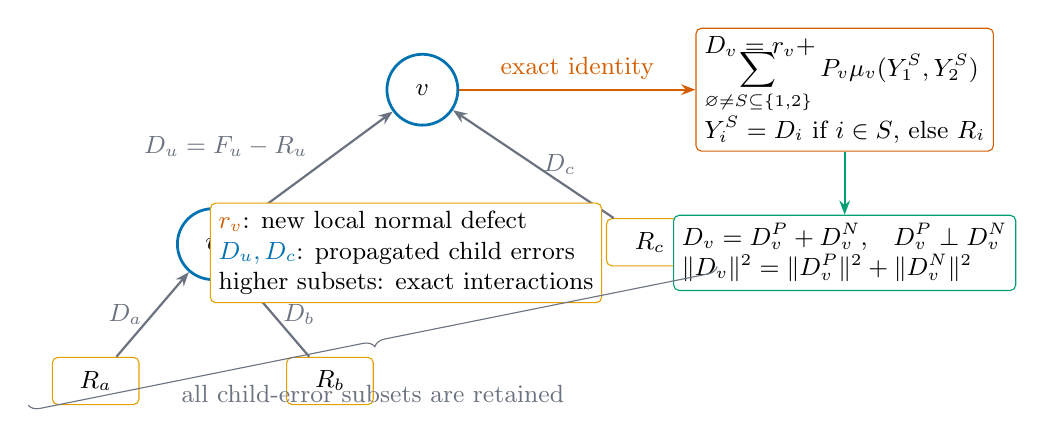
\begin{tikzpicture}[font=\small,node distance=9mm and 16mm]
  \node[nodeop] (v) {$v$};
  \node[nodeop,below left=13mm and 20mm of v] (u) {$u$};
  \node[leaf,below left=11mm and 6mm of u] (a) {$R_a$};
  \node[leaf,below right=11mm and 6mm of u] (b) {$R_b$};
  \node[leaf,below right=13mm and 20mm of v] (c) {$R_c$};
  \draw[edge] (a) -- node[left] {$D_a$} (u);
  \draw[edge] (b) -- node[right] {$D_b$} (u);
  \draw[edge] (u) -- node[above left] {$D_u=F_u-R_u$} (v);
  \draw[edge] (c) -- node[right] {$D_c$} (v);
  \node[note,draw=seionred,right=30mm of v] (identity) {
    $D_v=r_v+$\\[-1mm]
    $\displaystyle\sum_{\varnothing\ne S\subseteq\{1,2\}}$
    $P_v\mu_v(Y_1^S,Y_2^S)$\\
    $Y_i^S=D_i$ if $i\in S$, else $R_i$};
  \draw[edge,seionred] (v) -- node[above] {exact identity} (identity);
  \node[note,draw=seiongreen,below=8mm of identity] (orth) {
    $D_v=D_v^P+D_v^N$,\quad $D_v^P\perp D_v^N$\\
    $\lVert D_v\rVert^2=\lVert D_v^P\rVert^2+\lVert D_v^N\rVert^2$};
  \draw[edge,seiongreen] (identity) -- (orth);
  \node[note,draw=seionorange,left=9mm of orth] (sources) {
    \textcolor{seionred}{$r_v$}: new local normal defect\\
    \textcolor{seionblue}{$D_u,D_c$}: propagated child errors\\
    higher subsets: exact interactions};
  \draw[decorate,decoration={brace,mirror,amplitude=4pt},seiongray]
    ([xshift=-3mm]a.south west) -- ([xshift=3mm]c.south east)
    node[midway,below=5mm,seiongray] {all child-error subsets are retained};
\end{tikzpicture}
\end{document}
